\chapter{Theoretische Grundlagen}
%1. Theoretische Grundlagen → als Grundlage für Implementierung
% Was muss der Leser wissen, um die Realisierung zu verstehen? 
%1. Konkreter, technologischer: Worum geht es bei Plattformunabhängigkeit, wie ist zu erreichen? → verschiedene grundsätzliche Konzepte
%2. Übersicht / Eigenschaften & Einordnung der vorgestellten L\"osungen
%3. Verwendete Technologien → wie macht das phonegap?
%1. Knockout, jquerymobile, etc.

\section{Apps für mobile Geräte}

\subsection{Mobile (native) Apps} \label{sec:native}
Unter mobilen \glspl{app} versteht man im Allgemeinen Anwendungssoftware für Tablet-Computer oder Smartphones. 
Im Laufe der letzten Jahre haben sich auf dem Markt für Mobilgeräte durch viele konkurrierende Gerätehersteller eine Vielzahl von Smartphone- und Tablet-Betriebssystemen herausgebildet.
Im Entwicklungsbereich wird in dem Zusammenhang auch von \glspl{plattform} gesprochen.

Zu den \glspl{plattform} mit dem höchsten Marktanteil zählen \glspl{google} Betriebssystem \gls{android}, \gls{ios} von \gls{apple}, \gls{win-phone} und \gls{blackberry-os} des gleichnamigen Smartphone-Herstellers \gls{blackberry-inc} \cite{platforms-marketshare}.
% Nativ-Entwicklung für die jeweiligen Plattformen: Android / iOS
Die \gls{app}-Entwicklung für diese mobilen Betriebssysteme erfolgt mehr oder weniger ähnlich und soll im Folgenden, um auf die beiden größten Vertreter einzugehen, anhand von \gls{android} beziehungsweise \gls{ios} näher beschrieben werden.

%	-> \gls{sdk}s verwalten
Grundsätzlich müssen auf der \gls{ide} die entsprechenden \glspl{sdk} der \gls{plattform}, für die entwickelt wird, installiert sein. 
Diese enthalten Softwarekomponenten, die zur Entwicklung der \gls{app} notwendig sind, beispielsweise Klassen, die es einem erlauben, auf native Funktionalitäten des Betriebssystems wie zum Beispiel das Adressbuch, den Benachrichtigungsmechanismus oder auch auf Hardwarekomponenten wie die Kamera, den Bewegungssensor oder das \gls{gps}-Modul zuzugreifen sowie die entsprechenden plattformspezifischen Oberflächenkomponenten des jeweiligen \gls{gui}-Toolkits zu nutzen.

%	-> Code schreiben für die jeweilige Plattform
% Allgemein / Android
Als Programmiersprache für die \gls{android}-\gls{app}-Entwicklung wird \gls{java} verwendet. Das heißt, als Voraussetzung für die Entwicklung von \gls{android}-\glspl{app} ist lediglich eine geeignete \gls{ide} wie \gls{eclipse}, \gls{netbeans} oder \gls{intellij} sowie eine Installation des \gls{java}- und des \gls{android}-\gls{sdk} nötig. 
\todo{wie sieht es mit dem deployment, also der Auslieferung in appstores etc. aus?}
Seit 2013 bietet Google darüber hinaus die auf \gls{intellij} basierende und eigens für die \gls{android}-Entwicklung angepasste \gls{ide} \gls{android-studio} an \cite{android-studio}, die bereits alle notwendigen Toolkits enthält. 
Nachdem der Code geschrieben ist, kann er kompiliert und zu einem lauffähigen Programm \emph{gebaut} (engl. \enquote{build}) %TODO ins Glossar, allerdings eigentlich mit beugung und so
 werden (\seeref{fig:hybrid-apps-schaubild}). Anschließend kann die \gls{app} in dem für die Zielplattform vorgesehenen Dateiformat ausgeliefert und auf dem Zielgerät installiert werden.

% iOS: 
Auch der Software- und Computer-Hersteller Apple bietet mit \gls{xcode} eine firmeneigene \gls{ide} zur \gls{app}-Entwicklung für sein mobiles Betriebssystem \gls{ios} an. Anders als Google geht der iPhone-Hersteller hier allerdings etwas restriktiver vor. So läuft die \gls{ide} \gls{xcode}, die man für die native \gls{ios}-Entwicklung benötigt, nur unter dem hauseigenen Betriebssystem \gls{osx} und das wiederum nur auf den firmeneigenen Mac-Rechnern. So sichert sich Apple auch durch jeden Entwickler einen neuen Kunden. \todo{darf man so was hier anmerken, oder lieber weg?}
Ansonsten verläuft der Entwicklungsprozess bei der \gls{ios}-Entwicklung im Prinzip ähnlich zur \gls{android}-Entwicklung (\seeref{fig:hybrid-apps-schaubild}).
Als Programmiersprache wird \gls{obj-c} verwendet, einer um objektorientierte Elemente erweiterte Variante der Programmiersprache \gls{c}.

Möchte ein Auftraggeber einer Software also statt seinen Kunden nur eine \gls{app} für ein Betriebssystem anzubieten, einen größeren Nutzerkreis erschließen, muss die zu entwickelnde \gls{app} für jede Zielplattform neu programmiert, getestet und gebaut werden, da jede mobile \gls{plattform} ihre eigenen Toolkits, Bibliotheken und Programmiersprachen verwendet, was die native \gls{app}-Entwicklung für potenzielle Auftraggeber zu einem sehr kostenaufwändigen Projekt werden lassen kann.
Andererseits bietet die native \gls{app}-Entwicklung vollständige Unterstützung der betriebssystemeigenen Funktionalitäten wie den Zugriff auf Kamera, Adressbuch, Bewegungssensoren etc. der jeweiligen \gls{plattform}, sodass ein Softwareprojekt mit solchen besonders hardware- oder betriebssystemnahen Anforderungen die Entwicklung einer nativen (plattformspezifischen) \gls{app} notwendig erscheinen lassen kann.\footnote{Mehr dazu in \autoref{sec:hybrid-dev}}

\subsection{Web-Anwendungen}\label{sec:web-app}

% Zuerst gab es Websites, dann dynamische Websites
Eine \gls{web-app} ist eine Anwendungssoftware, die auf einem Web-Server läuft und auf die der Nutzer mittels eines Browsers zugreifen kann; also eine dynamische Website, wie man sie auch schon vor dem Aufkommen von Smartphones und modernen Tablets kannte. 

Die Grundlage für die Entwicklung von Internetseiten bildet der langjährige Standard \gls{html}, mit dem deren Aussehen, Inhalt und Struktur textuell beschrieben werden kann. 
In Kombination mit \gls{css} für die modulare Gestaltung einer Website sowie \gls{js}, einer Skriptsprache zur \gls{dom}-Manipulation, bietet die \gls{html}-Spezifikation in ihrer neusten Version \textit{(\gls{html5})} im Grunde alles, was für die Entwicklung einer modernen grafischen Benutzerschnittstelle notwendig ist. 
Die Fachlogik liegt, neben den Oberflächen-Komponenten in Form von \mbox{\gls{html}-,} \gls{css}- und Javascript-Dokumenten, auf einem Webserver und verarbeitet und reagiert auf Anfragen des Clients.\footnote{Die Rolle des Clients übernimmet hier also der Browser.}
Als Server-Technologie ist ein breites Spektrum an Programmiersprachen und Umgebungen einsetzbar.\footnote{Einige sind beispielsweise \gls*{php}, \gls*{java}, \gls*{asp} u.\,v.\,a.\,m.}

Somit bietet die Entwicklung einer \gls{web-app} (abgesehen von einigen Browser-spezifischen Eigenheiten) bereits eine gewisse Plattformunabhängigkeit, da jedes moderne Betriebssystem über einen Webbrowser verfügt. 
Zwar müssen Entwickler in bestimmten Details bei der Erstellung des Codes auf die teilweise unterschiedliche Unterstützung (bspw. von \gls{html}-Elementen) \todo{genauer?} durch die verschiedenen Browser achten, aber darüber hinaus wird der Entwicklungsaufwand für eine \gls{web-app} nicht von der Anzahl der Zielplattformen bestimmt, da von Client-Seite aus verschiedene Browser durch die Verbreitung und Beachtung von Web-Standards weitgehend einheitliche \gls{html}-Dokumente lesen und interpretieren können und das Back\-end nicht auf Clients mit unterschiedlichen \gls{plattform}en, sondern auf Webservern liegt, deren \gls{plattform} bei der Entwicklung entweder schon bekannt oder nicht relevant ist.\footnote{Beispielsweise weil auch die Fachlogik plattformunabhängig mit \gls*{php} oder \gls*{java} realisiert wurde.}

% Dann für sämtliche INet-Dienste auch noch eine \gls{app}
Obwohl es, durch damals eher im Business-Bereich verortete Internet-Handys und Palmtops, auch vor den heute üblichen mobilen Touch-Geräten bereits mobile Internetseiten gab, die speziell für die Darstellung auf kleinen Displays ausgerichtet waren, boten mit der massenhaften Verbreitung von mobilen, internetfähigen Geräten und deren (im Folgenden erläuterten) stark anwendungsorientierten Bedien-Konzepten viele herkömmliche Internet-Dienste nun auch zusätzlich eine native \gls{app} für verschiedene mobile \glspl{plattform} an.
So sind beispielsweise auch E-Mail-Dienste wie \gls{gmx}, \gls{web-de} oder \gls{gmail} seit der Verbreitung von Smartphones und Tablets auch in Form einer eigenen \gls{app} für \gls{android} und \gls{ios} vertreten, sodass der Nutzer, statt, wie von der Desktop-Computer-Nutzung gewohnt, einen anbieterunabhängigen Mail-Client zu konfigurieren, über den er seine E-Mails abruft, unter Umständen gleich die jeweilige \gls{app} des E-Mail-Anbieters startet \cite{gmx, web.de, gmail}.
Das heißt, der Nutzer folgt einem geänderten Bedienungsmuster seines Mobilgeräts gegenüber der herkömmlichen Computer-Nutzung: um zu einem bestimmten Ergebnis zu gelangen (bspw. \emph{Nachrichten lesen}) also die Frage zu beantworten, \emph{wie} er dahin gelangt (Einen Browser öffnen und zur gewünschten Seite navigieren: www.tagesschau.de), ist es für Anwender heutiger Mobilsysteme naheliegend, gleich die passende \gls{app} zu starten (Hier bspw. die Tagesschau-\gls{app}).

% Gründe für App statt Web-Anwendung
Dafür gibt es verschiedene mögliche Gründe. Zum Einen muss im Gegensatz zu einer Website bei der mobilen \gls{app} nicht die komplette Oberfläche\footnote{\gls{html}-, \gls{css}- und JavaScript-Dokumente sowie Grafiken} übertragen werden, sondern lediglich die Nutzdaten,\footnote{Also beispielsweise, um beim obigen Beispiel zu bleiben, die Nachrichten in Textform.} was dem Nutzer ein höheres Maß an Performanz einbringt.
Zum Anderen können trotz Vollbildmodus in bestimmten Fällen \gls{gui}-Elemente des Webbrowsers bei der Benutzung einer Web-Anwendung störend sein, so ist beispielsweise die Adresszeile am Rand nicht unbedingt erwünscht, wenn der Nutzer statt im Internet zu surfen dort eigentlich eine bestimmte Anwendung nutzen möchte. 
Ein anderes Beispiel für ein eventuell unerwünschtes Verhalten der Benutzerschnittstelle ist das der \emph{Menü}-Taste bei \gls{android}-Geräten, die im Falle der Nutzung einer Web-Anwendung über den Browser nicht den Kontext der eigentlich benutzten Anwendung anzeigt,\footnote{hier also der Website} sondern lediglich den des Browsers.

In bestimmten Fällen kann eine nützliche Funktion einer \gls{app} die Offline-Nutzung sein, wenn beispielsweise durch die abgedeckten Anwendungsfälle keine Verbindung oder Synchronisation mit einem Server nötig ist. Beispiele hierfür könnten, um nur einige zu nennen, ein Taschenrechner, kleine Spiele, oder eine Bildverarbeitungs-\gls{app} sein. 
Für diese Offline-Nutzung einer \gls{app} zeichnet die Web-Anwendung ein geteiltes Bild: Zwar wurden in den letzten Jahren mehrere Methoden entwickelt, eine Web-Anwendung auch offline nutzen zu können, doch durch ihre Ausrichtung auf die Nutzung via Internet stellt die Implementierung dieser Funktionalität für Entwickler einen Zusatzaufwand dar. 

Einige Möglichkeiten, eine Web-Anwendung ohne Internetverbindung nutzbar zu machen, sind beispielsweise die aus der \gls{html5}-Spezifikation hervorgehenden Technologien \gls{webstorage}, ein Mechanismus zum lokalen Speichern von größeren Datenmengen in Form von Schlüssel-Wert-Paaren \cite{w3c_webstorage} sowie \gls{websql} bzw. \gls{indexed-db}, beides auf Web-Anwendungen optimierte Datenbanken-Spezifikationen, die vom \gls{w3c} herausgegeben werden \cite{w3c_websql, w3c_indexedDB}.
Allerdings bestehen auch bei diesen Mechanismen teilweise Einschränkungen durch die Browservielfalt beziehungsweise deren Versionen. So wird \gls{indexed-db} beispielsweise nicht von \gls{safari} oder \gls{ios} unterstützt, \gls{chrome} muss für die Nutzung mindestens in Version 23 oder höher vorliegen, \gls{firefox} in 10 oder höher. 
Auch bei \gls{websql} zeichnet sich ein ähnlich diffuses Bild ab: Während \gls{chrome} die Technologie ab der Version 4 und \gls{ios} ab Version 3.2 unterstützt, ist für Nutzer der Browser \gls{firefox} und \gls{ie} die Technik gar nicht verfügbar.
Lediglich \gls{webstorage} wird weitgehend von allen gängigen Browsern unterstützt \cite{html5-rocks_offline}.
Weiterhin wird die Offline-Funktionalität gegenüber der nativen \gls{app} dadurch eingeschränkt, dass der Nutzer diese ohne weiteres Zutun des Entwicklers nur dann nutzen kann, wenn die entsprechende Internet-Seite im Offline-Zustand des Geräts bereits im Browser geöffnet ist, da diese nicht lokal auf dem Gerät, sondern auf einem Webserver gespeichert ist.
Für vollständigen Offline-Zugriff müsste der Entwickler die komplette Website so paketieren, dass der Nutzer sie -- wie eine native App -- von seinem Gerät aus starten und nutzen kann.\footnote{\seeref{sec:hybrid-app} und \ref{sec:hybrid-dev}.}

Allgemein kann man sagen, dass der Zugriff auf native Funktionalitäten des Geräts respektive des Betriebssystems nicht oder nur gering unterstützt wird, sodass der geringere Entwicklungsaufwand einer solchen \gls{web-app} (\seename~ \autoref{fig:hybrid-apps-schaubild}) unter Umständen zu Lasten des Funktionsumfangs und der Usability der Anwendung geht.
\todo{recherchieren: wird was unterstützt? gibt es Möglichkeiten, per Javascript etc.? Was wird \enquote{gering} unterstützt? sollte man das noch weiter ausführen? Touch-Gesten etc.?}

\subsection{Hybride Apps} \label{sec:hybrid-app}

Die \gls{hybrid-app} verbindet Eigenschaften der Nutzung einer nativen \gls{app} mit den Vorteilen der Web-Entwicklung mithilfe von Web-Technologien und entsprechenden Frameworks und löst damit beispielsweise das Problem der mangelnden Offline-Fähigkeit einer \gls{web-app} sowie deren geringe Unterstützung von plattformspezifischen oder hardware-nahen Funktionalitäten. 
Da jedes moderne mobile Betriebssystem für Entwickler auch die Möglichkeit bietet, eine Web-View in die zu entwickelnde App einzubinden, also eine \gls{gui}-Komponente, in die \gls{html}-Inhalte hinein geladen werden können, liegt der Ansatz für hybride Apps auf der Hand: Auf Entwicklungsebene wird die Anwendung als Web-App entwickelt, gleichzeitig mithilfe von entsprechenden APIs und Frameworks zur Anbindung an die native Ebene der Zielplattform in eine App für die jeweiligen \glspl{plattform} integriert, sodass auf Benutzerseite die Nutzung einer Web-Anwendung, die in puncto Funktionsumfang, Usability und Look-And-Feel einer nativen mobilen App sehr nahe kommt, möglich wird.

Dieses Vorgehen bietet unter anderem für Web-Entwickler den Vorteil, ihre bisherigen Programmierkenntnisse im Web-Bereich im Wesentlichen auch für die Entwicklung von hybriden \glspl{app} nutzen zu können. 
So wird in der Regel der grundlegende Teil des Codes für das Frontend, wie bei der Web-Entwicklung, in \gls{html} in Kombination mit \gls{css} und \gls{js} geschrieben und getestet. 
Da allerdings auf dem mobilen Gerät für das Backend, also die Verarbeitungsinstanzen, nicht, wie bei einer herkömmlichen Web-Anwendung, ein Server mit einer entsprechenden Server-Technologie wie \gls{php} oder \gls{asp} läuft, wird auch dieser Teil der App bei der hybriden Entwicklung meist mit \gls{js} bewerkstelligt. 
\todo{recherchieren! Kann man Perl oder Python oder so auf einem Android laufen lassen?}
Anschließend muss die Anwendung für die verschiedenen Zielplattformen gebaut werden, um in das jeweilige Container-Format für Apps der verschiedenen \glspl{plattform} eingebunden werden zu können und den Zugriff auf die plattformspezifischen Toolkits durch die Cross-Platform-APIs zu ermöglichen (\autoref{fig:hybrid-apps-schaubild}).
Hierfür kann es erforderlich sein, dass auf der Entwicklungsplattform die jeweiligen \glspl{sdk} installiert sind, was gegenüber der Web-Entwicklung einen administrativen Mehraufwand darstellt.
Eine andere Variante ist die Auslagerung des Bauprozesses auf einen externen Build-Server, beispielsweise mithilfe eines externen Web-Service eines Drittanbieters, was den Vorteil hat, die \glspl{sdk} für die Zielplattformen nicht auf jedem Entwicklungsrechner verwalten zu müssen. 
Allerdings hat der Entwickler durch die Herausgabe des Codes an einen solchen Dienstleister nicht mehr die vollständige Kontrolle über den Code, sodass die Variante der Auslagerung des Build-Prozesses gerade für Closed-Source-Projekte unter Umständen nicht in Frage kommt. 
Des Weiteren kann der Betreiber des Build-Services unter Umständen Restriktionen bezüglich der Plattformunterstützung erteilen, wodurch eventuell eine geringere Anzahl von Zielplattformen unterstützt wird, als von Entwicklerseite gewünscht oder erfordert.\footnote{Beispielsweise unterstützt \gls{pg-build} in der neusten Version 3 nur nur noch die drei großen Mobilplattformen \gls{android}, \gls{ios}, und \gls{win-phone}.}

%TODO Gibts hierfür auch so ne Art Grafik-Datenbank wie bei Bib? Dann müsste man den schmonsens nicht hier im Text verteilen.
%TODO Wie gibt man hier ne Bild-Quelle an?
	%TODO Eine Referenz für die Grafik (von mir) und alle Referenzen der verwendeten Bilder?
%TODO Positionierung!
%TODO Grafiken ohne fileextension
%TODO Eigenschaften wie Größe etc. zentral definieren statt in jedem Bild!!
\begin{figure}[h!]
\centering
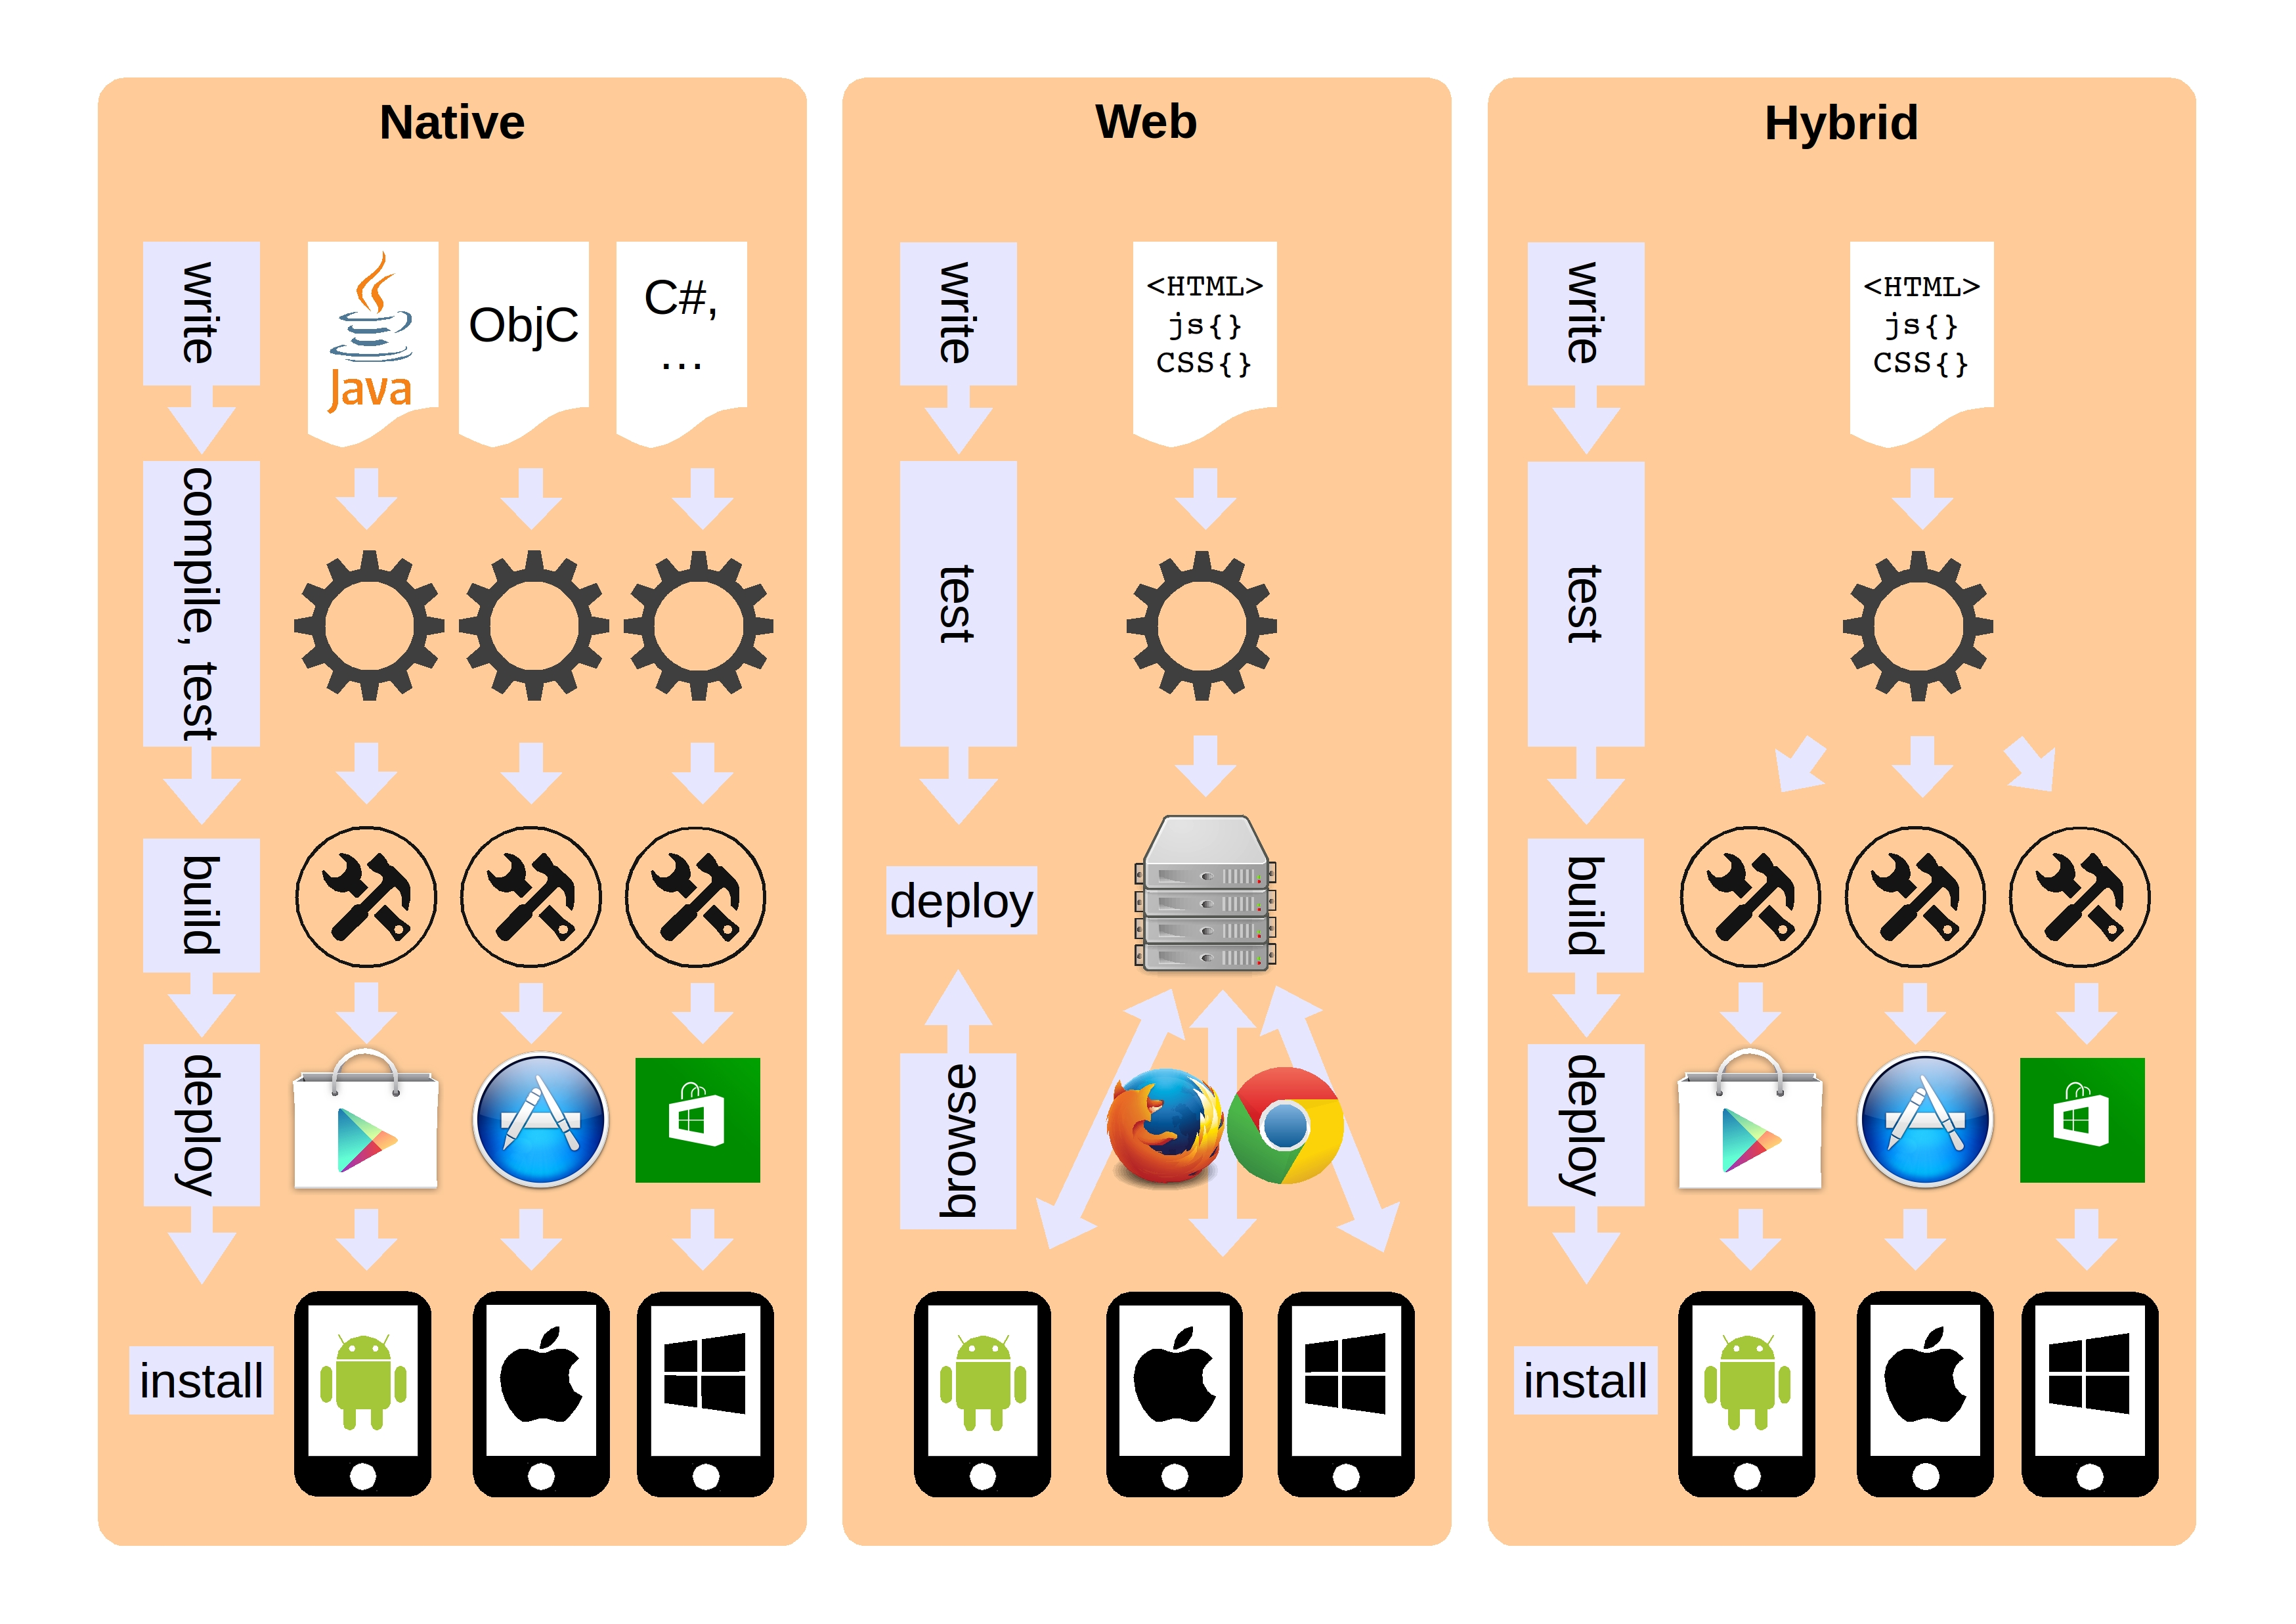
\includegraphics[
	width=1\textwidth,
	natwidth=1,
	natheight=1
	]{hybrid-apps-schaubild}
	\caption
		[Schaubild Hybrid Apps]
		{Entwicklungsstufen der verschiedenen Arten von \glspl{app}. Während bei der nativen \gls{app} der gesamte Entwicklungszyklus einmal pro \gls{plattform} durchlaufen werden muss, verringert sich der Aufwand für die \gls{web-app} erheblich. Bei der \gls{hybrid-app} muss die Anwendung zwar einmal für jede \gls{plattform} gebaut und ausgeliefert werden, um die Schnittstellen für die nativen \glspl{plattform} zu implementieren, aber der hauptsächliche Entwicklungsaufwand des Programmierens und Testens fällt aufgrund des generischen Charakters nur einmal an.}
	\label{fig:hybrid-apps-schaubild}
	\imagesourcefont
	\vspace{\imagesourcespace}
	\imagesourcefont{}
	\caption*{\imagesourcelabel Eigene Grafik.}
\end{figure}


\begin{comment}
%TODO Ein Andermal, wenn noch Zeit ist....

\section{Plattformunabhängige App-Entwicklung}

%\subsection{Möglichkeiten des Erreichens von Plattformunabhängigkeit}

\subsection[Lösungen]{Lösungen für die plattformunabhängige App-Entwicklung}
%TODO Ergebnisse aus GoogleDocs-Recherche Zusammentragen

[\ldots]%TODO Fertig schreiben

%TODO Gibts es andere Ansätze als den hybriden?

%TODO Lösungen beschreiben und Ansätze kurz erläutern
%TODO Titanium
%TODO PhoneGap
%TODO Appcelarator
%TODO etc.

\end{comment}

\section{Entwicklung von hybriden Apps}\label{sec:hybrid-dev}

Wie in \ref{sec:hybrid-app} beschrieben, bildet die hybride App-Entwicklung die Schnittmenge aus der nativen App-Entwicklung und der Web-Entwicklung mithilfe von Web-Technologien und zusätzlichen Frameworks und Bibliotheken. 
Hier soll mit \gls{cordova}\,/\,\gls{phonegap} die konkrete Nutzung eines dieser Frameworks und weitere verwendete Technologien wie \gls{ko} oder \gls{jqm} erläutert werden.

\subsection{JQuery}

Bereits für die Entwicklung von reinen Web-Anwendungen stellen neben den grundlegenden Web-Technologien \gls{html}, \gls{css} und \gls{js} Erweiterungen wie die JavaScript-Bibliothek \gls{jq} nützliche Hilfsmittel dar, die viele Funktionen gegenüber der Verwendung von \enquote{reinem} \gls{js} deutlich vereinfacht.
So ist beispielsweise der Programmieraufwand für den Zugriff auf Elemente einer \gls{html}-Seite durch \gls{jq} wesentlich geringer als ohne die Bibliothek.
Besonders deutlich wird dies an den unten aufgeführten Code-Beispielen, in denen ein Button exemplarisch die Funktionalität übernehmen soll, alle Absätze einer \gls{html}-Seite auszublenden.
Während bei herkömmlichem \gls{js} für die Selektion aller Elemente die Funktion \lstinline|getElementsByTagName()| aufgerufen werden muss (\seeref{lst:js}), ist bei \gls{jq} der Zugriff auf alle Elemente eines \glspl{tag} per Dollar(\lstinline|$|)-Notation deutlich verkürzt (\seeref{lst:jq}).
Auch die nächste Anweisung zur Ausführung einer Operation für alle ausgewählten Elemente (hier: \lstinline|hide()|, also \textit{ausblenden}) fällt bei \gls{jq} wesentlich kürzer aus, indem die Funktion noch in der selben Zeile wie der vorherigen Selektor aufgerufen werden kann (\lstinline|$("p").hide();|).
Bei der reinen \gls{js}-Variante ist nach der Selektion aller Absätze zunächst einmal ein Array ausgewählt, sodass, um auf den einzelnen Elementen Operationen ausführen zu können, durch alle Elemente des Arrays iteriert und die Funktion für jedes Element aufgerufen werden muss (\seeref{lst:js}, \linenamepl 5\,-\,7).

%TODO Zentral definieren!!
\par\noindent\begin{minipage}{\linewidth}
\lstinputlisting[
	label=lst:jq,
	style=htmlcssjs, 
	caption=\gls{jq}-Beispiel-Code zum Ausblenden aller Absätze \cite{w3schools_jq_hide}.,
	]{code/jquery.html}
\end{minipage}\par\addvspace{\topskip}

\par\noindent\begin{minipage}{\linewidth}
\lstinputlisting[
	label=lst:js,
	style=htmlcssjs, 
	caption=Die selbe Funktionalität wie in \autoref{lst:jq} mit reinem \gls{js}.,
	]{code/without-jquery.html}
\end{minipage}\par\addvspace{\topskip}
	
\subsection{Knockout} \todo{evtl. andere Überschriften} \label{ko}

Neben \gls{jq} bietet das \gls{ko}-Framework ein weiteres nützliches Hilfsmittel für die Entwicklung von Web-Anwendungen, das ebenso wie \gls{jq} und \gls{jqm} aus einer \gls{js}-Bibliothek besteht und die Verbindung der \gls{html}-Oberfläche mit der Programmlogik der Anwendung mittels \gls{data-binding}, also der dynamischen Anbindung von \gls{ui}-Komponenten zu Datenfeldern auf Programmebene, erheblich vereinfacht.
Das \gls{data-binding} wird bei \gls{ko} durch das \gls{mvvm}-Pattern realisiert, das Entwicklern eine Trennung zwischen Benutzeroberfläche und \gls{ui}-Logik ermöglicht.
Diese Aufteilung dient unter anderem der Übersichtlichkeit des Codes und kann beispielsweise die Aufteilung der Entwicklung von Benutzerschnittstellen erleichtern, indem die \gls{ui}- und die Geschäftslogik von Softwareentwicklern übernommen werden kann, während Designer den Schwerpunkt auf die Gestaltung der Oberfläche legen können \cite{Model_View_ViewModel__Wikipedia}.

\begin{figure}[h!]
\centering
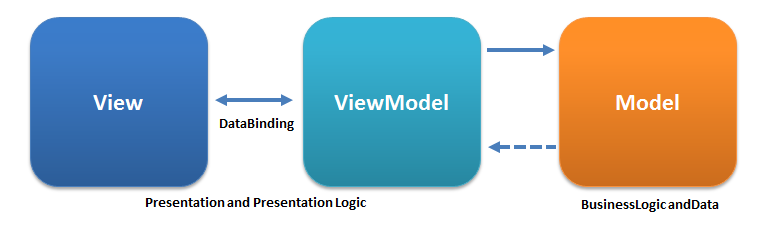
\includegraphics[
	width=1\textwidth,
	natwidth=1,
	natheight=1
	]{mvvm-pattern}
\caption[\gls{mvvm}-Pattern]{Schematische Darstellung des Entwurfsmusters \gls{mvvm}: Die View ist über das \gls{data-binding} mit dem ViewModel verbunden, indem die \gls{ui}-Logik implementiert ist und das mit der Geschäftslogik (Model) interagiert.}
\label{fig:mvvm-pattern}
	\imagesourcefont
	\vspace{\imagesourcespace}
	\imagesourcefont{}
	\caption*{\imagesourcelabel Wikimedia Commons \cite{MVVMPattern}.}
\end{figure}

Das \gls{mvvm}-Pattern stellt eine Gliederung der Software in drei Grundlegende Komponenten dar:
Die \gls{view} Repräsentiert die Präsentationsschicht, also die Benutzeroberfläche, im Falle der Web-Anwendung also die \gls{html}-Seite, deren Elemente per \gls{data-binding} an Eigenschaften des \glspl{view-model} gebunden werden können. 
Das \gls{model} steht für die Geschäftslogik und beinhaltet das Datenmodell und die Funktionen, die vom \gls{view-model} angefragt werden können, um beispielsweise Benutzereingaben zu validieren oder Daten für die Anzeige in der Oberfläche zu erhalten (\seeref{fig:mvvm-pattern}).

Ein wesentlicher Menchanismus für die Aktualisierung der Oberfläche bei einer Änderung des \glspl{view-model} von \gls{ko} ist die Verwendung von \glspl{obs}, also Objekten oder Datenfeldern, welche bei Änderungen ihres Inhalts eine Nachricht aussenden, sodass andere Objekte automatisch auf die Zustandsänderung des \glspl{obs} reagieren können, beispielsweise, um die Anzeige auf der Oberfläche zu aktualisieren.

Im Code-Beispiel unten (\autoref{lst:ko}) wird ein einfaches \gls{view-model} mit drei Eigenschaften erstellt: \lstinline|firstName|, \lstinline|lastName|, und \lstinline|fullName|, wobei die ersten beiden \emph{\glspl{obs}} darstellen und letztere aus den anderen beiden Feldern generiert wird (\linenamepl 10\,-\,13).
Durch den Aufruf der \gls{ko}-Funktion \lstinline|observable()| ist es nicht notwendig, bei einer Änderung der Daten an der Oberfläche, die Änderung der Anzeige der Daten (\linename 27) explizit anzustoßen (Beispielsweise per EventListener auf einer \gls{ui}-Komponente).
Stattdessen übernimmt das \gls{ko}-Framework die Durchreichung aller Änderungen im \gls{view-model}, sodass bei einer Benutzereingabe in eines der \lstinline|<input>|-Felder eine Änderung der Daten im \gls{view-model} registriert wird und automatisch alle damit verbundenen \glspl{view} aktualisiert werden (\seeref{fig:ko-hello-world}).\footnote{Hier das \texttt{<h2>}-Element, das mit der \gls{view-model}-Eigenschaft \texttt{fullName} verknüpft ist.}

\par\noindent\begin{minipage}{\linewidth}
\lstinputlisting[
%	float,floatplacement=H,
	label=lst:ko,
	style=htmlcssjs, 
	caption=Einfaches Anwendungsbeispiel für die Verwendung der \gls{js}-Bibliothek \gls{ko}.,
	]{code/ko.html}
\end{minipage}\par\addvspace{\topskip}

\begin{figure}[h!]
\centering
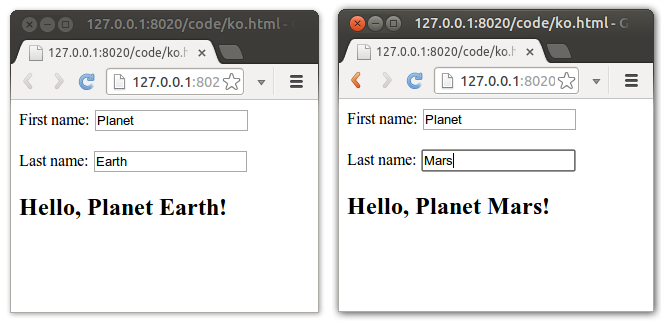
\includegraphics[
	width=1\textwidth,
	natwidth=1,
	natheight=1
	]{ko-hello-world}
	\caption
		[\gls{ko}-Beispiel im Browser.]
		{\gls{ko}-Beispiel aus \autoref{lst:ko} im Browser. Links im Bild: Anzeige bei Initialisierung der Oberfläche, rechts: Benutzereingabe ins Eingabefeld: \enquote{Mars}. \\ Änderungen in der \gls{ui} (Hier: im Eingabefeld) werden sofort im \gls{view-model} registriert und automatisch an alle verknüpften Anzeigen weitergereicht (Hier an das fettgedruckte Begrüßungselement).}
	\label{fig:ko-hello-world}
	\imagesourcefont
	\vspace{\imagesourcespace}
	\imagesourcefont{}
	\caption*{\imagesourcelabel Eigener Screenshot.}
\end{figure}

\subsection{JQuery\,Mobile}

Um das Erscheinungsbild und Verhalten von Webseiten an eine bessere Benutzung für mobile Geräte anzupassen, bietet sich der Einsatz eines entsprechenden \gls{gui}-Toolkits an. 
Die von der \gls{jq-foundation} entwickelte \gls{gui}-Bibliothek \gls{jqm} bietet hier Möglichkeiten für Entwickler von mobilen Webseiten, ihre Dokumente an verschiedene Eigenschaften anzupassen, die gemeinhin unter dem Begriff \gls{laf} zusammengefasst werden, wie dem äußeren Erscheinungsbild, der Fähigkeit, mit Touch-Gesten umzugehen, der Anpassung an die geringere Display-Größe sowie von vielen mobilen \glspl{app} gewohnten Animationen, und somit erwartungskonform zu gestalten.

\Gls{jqm} besteht mit einer \gls{js}-Bibliothek und einem zusätzlichen Stylesheet in \gls{css}, aus zwei Dokumenten, deren Einbindung in die \gls{html}-Seite analog zu der von \gls{jq} per Verlinkung als \lstinline|<script>|- beziehungsweise \lstinline|<link>|-\gls{tag} funktioniert.
Da \gls{jqm} auf \gls{jq} aufbaut, muss auch der Link zum \gls{jq}-Script gesetzt sein, um auf die benötigten Funktionen zugreifen zu können (\seeref{lst:jqm}, \linenamepl 3\,-\,5).

\par\noindent\begin{minipage}{\linewidth}
\lstinputlisting[
%	float,floatplacement=H,
	label=lst:jqm,
	style=htmlcssjs,
	caption=Einbindung von \gls{jqm} in eine \gls{html}-Seite \cite{w3schools_jqm_start}.,
	]{code/jquerymobile.html}
\end{minipage}\par\addvspace{\topskip}
	
Die Definition von \gls{gui}-Elementen geschieht hierbei über das \gls{html}-Attribut \lstinline|data-role|, dem vordefinierte Werte wie \lstinline|page|, \lstinline|header|, \lstinline|footer|, \lstinline|button| u.\,v.\,a.\,m. zugeteilt werden können, anhand derer das \gls{jqm}-Framework den \gls{html}-Elementen die jeweilige Style-Definition aus dem Stylesheet zuweisen kann (\seeref{lst:jqm}, \linenamepl 8, 9, 12 und 15).
Somit wird dem Entwickler ermöglicht, ohne zusätzlichen Entwicklungsaufwand für die Programmierung von \gls{gui}-Komponenten oder Erstellung von Style-Definitionen Webseiten mit zeitgemäßem und adäquaten \gls{laf} für mobile Geräte anzupassen (\seeref{fig:jqm} und \ref{fig:without-jqm}).

Neben der Zuweisung von Rollen über das \lstinline|data-role|-Attribut, durch die das Framework den \gls{gui}-Komponenten automatisch entsprechende Style-Definitionen zuweist, können weiterhin über das \lstinline|class|-Attribut direkt Style-Klassen aus dem \gls{jq}-Stylesheet verwendet werden.
Beispielsweise sorgt im obigen Beispiel der Zusatz \lstinline|class="ui-content"| (\autoref{lst:jqm}, \linename 12) für ein besseres Layout des \lstinline|<div>|-Inhalts, wie der Vergleich ohne das \lstinline|class|-Attribut in \autoref{fig:without-ui-content-class} zeigt.

\begin{figure}[h!]
\centering
	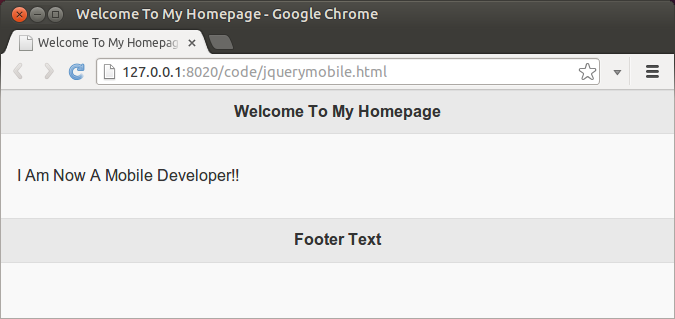
\includegraphics[
	width=1\textwidth,
	natwidth=1,
	natheight=1
	]{jqm}
	\caption[\gls{jqm}-Beispiel]{\gls{jqm}-Beispiel aus \autoref{lst:jqm} im Browser.}
	\label{fig:jqm}
	\imagesourcefont
	\vspace{\imagesourcespace}
	\imagesourcefont{}
	\caption*{\imagesourcelabel Eigener Screenshot.}
\end{figure}

\begin{figure}[h!]
\centering
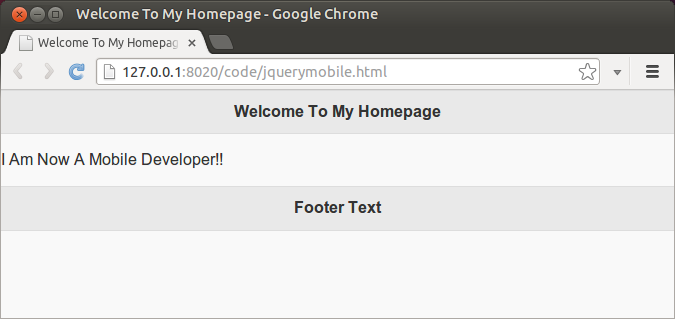
\includegraphics[
	width=1\textwidth,
	natwidth=1,
	natheight=1
	]{without-ui-content-class}
	\caption[Beispiel ohne class-Attribut]{Beispiel-Oberfläche wie in \autoref{fig:jqm}, ohne das class-Attribut in \autoref{lst:ko}, \linename 12.}
	\label{fig:without-ui-content-class}
	\imagesourcefont
	\vspace{\imagesourcespace}
	\imagesourcefont{}
	\caption*{\imagesourcelabel Eigener Screenshot.}
\end{figure}

\begin{figure}[h!]
\centering
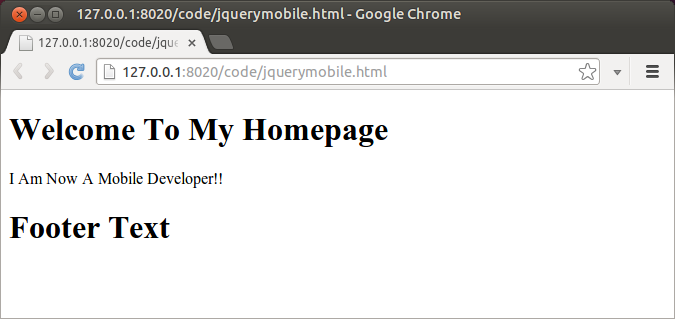
\includegraphics[
	width=1\textwidth,
	natwidth=1,
	natheight=1
	]{without-jqm}
	\caption[Beispiel ohne \gls{jqm}]{Beispiel-Oberfläche wie in \autoref{fig:jqm}, aber ohne die \gls{jqm}-Bibliotheken.}
	\label{fig:without-jqm}
	\imagesourcefont
	\vspace{\imagesourcespace}
	\imagesourcefont{}
	\caption*{\imagesourcelabel Eigener Screenshot.}
\end{figure}

\subsection{Phonegap\,/\,Cordova} \label{sec:phonegap}

% Vorstellung ----------------------------------------------

\gls{phonegap} ist ein \gls{opensource}-Framework von \gls{adobe} zur Erstellung von hybriden \glspl{app} und bildet damit die Grundlage für den hier explorierten Ansatz zur plattformunabhängigen \gls{app}-Entwicklung.
Die Software wurde ursprünglich unter dem Namen \gls{phonegap} von der Firma \gls{nitobi} entwickelt, die 2011 von \gls{adobe} aufgekauft wurde \cite{Adobe_Announces_Agreement_to_Acquire_Nitobi_Creator_of_PhoneGap}. 
Später wurde die Code-Basis der \gls{apache} übergeben und dort in \gls{cordova} umbenannt, wodurch das Framework in den Quellen stellenweise unter beiden Namen erscheint.
\Gls{adobe} \gls{phonegap} baut also als dessen Distribution auf \gls{cordova} auf, wobei derzeit der einzige wesentliche Unterschied im Namen des Pakets besteht (Stand: \citedate{PhoneGap_Cordova_and_whats_in_a_name}), nach eigenen Angaben aber durchaus weitere Tools mit Bezug auf andere \gls{adobe}-Dienste in die \gls{phonegap}-Distribution einfließen können \cite{PhoneGap_Cordova_and_whats_in_a_name}.

Da das \gls{apache}-Framework als \gls{opensource}-Basis auch die allgemeine Grundlage für weitere \gls{cordova}-Distributionen bildet und so auch die Community-Anlaufstelle zur Mitwirkung am \gls{cordova}-Projekt darstellt~\cite{PhoneGap_Cordova_and_whats_in_a_name}, wird im Folgenden weitgehend der Begriff \enquote{\gls{cordova}} verwendet, die meisten Inhalte treffen aber ebenso auf die \gls{adobe}-Version \gls{phonegap} zu. \todo{Oder ist das nicht eigentlich eh klar, da Cordova du \emph{Grundlage} bildet?}
%TODO Nach praktischem Teil nochmal checken!

% Beschreibung / Übersicht: Komponenten --------------------

Wie in \autoref{sec:hybrid-app} beschrieben, wird bei der hybriden App-Entwicklung eine Web-App programmiert, die dann in eine native WebView "verpackt" werden kann und somit auf dem jeweiligen Monbilgerät alsl mobile App ausgeführt werden kann. 
Das \gls{cordova}-Framework besteht darüberhinaus im Wesentlichen aus einer \gls{api} in Form einer \gls{js}-Bibliothek, die es dem Entwickler ermöglicht, auf native Funktionaltitäten des mobilen Betriebsystems zuzugreifen sowie einem mitgelieferten \gls{cli}, das für die Erstellung, Erweiterung und Anpassung der Anwendung, zur Bewerkstelligung des Build-Prozesses für die verschiedenen Plattformen sowie auch der Ausführung in einem Emulator oder auf einem Mobilgerät zum Testen der Anwendung dient \cite{Cordova-Docs_Overview}.

% Entwicklungsworkflows ------------------------------------

In der Cordova-Dokumentaiton werden zwei grundlegende Entwicklungsszenarien beschrieben, für die das Framework verwendet werden kann. 
Mit der Version 3.0 wurde das cli Teil des Software-Paktes, das viele Arbeitsschritte automatisiert ausführt und damit den Cordova-Entwicklungsprozess vereinfacht. 
Der Hauptfokus dieses Wekrzeugs liegt im für die hybride App-Entwicklung grundlegenden Entwicklungsworkflows, oder auch emph{Web-Entwicklungsansatz}.
Dieser Ansatz bietet die breiteste Plattformunterstützung bei möglichst geringem Mehraufwand für unterschiedliche Plattformen und damit den hier hauptsächlich fokussierten Ansatz \cite{Cordova-Docs_CLI}.

Soll nur eine bestimmte Zielplattform bedient werden, kann auch nach dem \emph{Nativen-Plattformansatz} entwickelt werden.
Dieser kann bspw. sinnvoll sein, wenn Entwickler mobiler Apps ihre Kenntnisse im Web-Bereich für die Entwicklung mobiler Apps nutzen möchten und sehr plattformspezifische Eigenschaften angepasst werden sollen, ist aber aufgrund des Mangels an entsprechenden Tools nicht oder nur gering für die Entwicklung plattformunabhängiger apps geeignet. 
Dabei wird das \gls{cli} in erster Linie für die Erstellung des Grundgerüsts der App verwendet, dessen Web-Teil dann mithilfe einer entsprechenden \gls{ide} in Kombination mit einem SDK der jeweiligen Plattform weiter verarbeitet und kompiliert werden kann \cite{Cordova-Docs_CLI}. 

% Plattform- / Feature-Unterstützung -----------------------

\begin{figure}[h!]
\centering
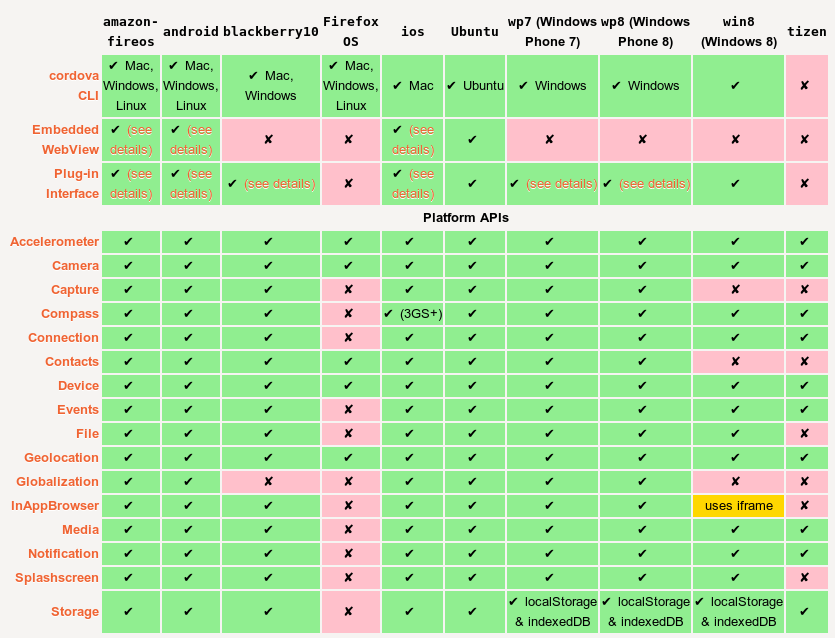
\includegraphics[
	width=1\textwidth,
	natwidth=1,
	natheight=1,
	]{cordova-platform-support}
	\caption
	[\gls{cordova} Plattform- und Feature-Unterstützung]
	{Plattform- und Feature-Unterstützung des \gls{cordova}-Frameworks: \\ 
	Bis auf wenige (\enquote{kleinere}) mobile Betriebssysteme bietet \gls{cordova} mit auch über die am weitesten verbreiteten Plattformen wie \gls{android}, \gls{ios} und \gls{win-phone} hinaus die volle Feature-Unterstützung für \gls{amazon-fireos}, \gls{ubuntu-phone} und eine fast vollständige für \gls{blackberry-os}.\\
	Für Entwickler von hybriden \glspl{app} dürfte hier auch vor allem die erste Zeile \emph{cordova CLI} interessant sein, da durch die Kompatibilität der jeweiligen Plattform-\glspl{sdk} nur bestimmte Kombinationen von Entwicklungs- und Zielplattform möglich sind.
	%TODO Erläuternden Text bspw. hier rein.
	}
	\label{fig:cordova-platform-support}
		\imagesourcefont
		\vspace{\imagesourcespace}
		\imagesourcefont{}
		\caption*{\imagesourcelabel Screenshot aus der \gls{cordova}-Dokumentation \cite{Cordova-Docs_Platform-Support}.}
\end{figure}


% Voraussetzungen ------------------------------------------

\gls{cordova} stellt für die Verwendung von nativen Funktionalitäten des mobilen Betriebssystems mit seiner \gls{js}-Plattform-\gls{api} eine Verbindung von der Web-Anwendungsebene zu den jeweiligen SDKs der Zielplattformen her.
somit müssen, um mit auf plattformspezifische Features zugreifen zu können, auf der Entwicklungsplattform alle \glspl{sdk} der gewünschten Zielplattformen installiert sein.
Da die \glspl{sdk} jedoch teilweise nur von bestimmten Desktop-Betriebssystemen unterstützt werden, muss das \gls{cli} unter Umständen auf mehreren Rechnern ausgeführt werden, die jeweils nur bestimmte mobile Plattformen bedienen (\seeref{fig:cordova-platform-support}).

% Funktionsweise -------------------------------------------

Nachdem das \gls{cordova}-Framework auf dem Entwicklungsrechner installiert ist, kann mit dem \gls{cli} ein neues App-Projekt angelegt werden. 
Dazu muss auf der Kommandozeile in das Entwicklungsverzeichnis für das zu erstellende Projekt navigiert werden und der das Cordova-Tool mit dem \lstinline|create|-Befehl aufgerufen werden (\seeref{lst:create}).

\begin{lstlisting}[
	language=bash,
	caption={Befehl zum erstellen einer Cordova-App.},
	label=lst:create]
	$ cordova create hello-beuth de.beuth-hochschule.hello HelloBeuth
\end{lstlisting}

Das erste Argument \lstinline|hello-beuth| spezifiziert dabei den Namen des Ordners für das zu erstellende App-Projekt, der mit dem \lstinline|create|-Befehl angelegt wird.
Der zweite und dritte Parameter sind optional und geben mit der \gls{id} in der wückwärts geschriebenen Domain-Bezeichnung und dem Namen ({\mbox{\enquote{HelloBeuth}}), der später für die App angezeigt wird, weitere Informationen für die App an, die einer \gls{xml}-Datei im neu angelegten Projekt-Ordner hinterlegt werden \cite{Cordova-Docs_CLI}.

Dabei erstellt das Tool in einem neuen Ordner ein Grundgerüst für die \gls{app}, das die nötige Struktur für den weiteren Entwicklungsprozess enthält (\seeref{fig:cordova-directory}).
Auf oberster Ebene liegt die Konfigurationsdatei \filename{config.xml}, in der grundlegende Eigenschaften sowie Informationen für den Build-Prozess hinterlegt werden können (\seeref{lst:config.xml}).
Daneben werden unter anderem (zu diesem Zeitpunkt noch leere) Ordner für Plugins und plattformspezifischen Code sowie ein \filename{www}-Ordner angelegt, der das Grundgerüst für den Web-Teil der \gls{hybrid-app} beinhaltet.
Neben der Datei \filename{index.html}, die die Beschreibung der Web-Oberfläche für die Anwendung darstellt werden nach üblichen Konventionen in der Webentwicklung weiterhin die Unterordner \filename{js}, \filename{css} und \filename{img} angelegt, worin die zur \gls{app} gehörigen \gls{js}- und \gls{css}-Dateien bzw. Bilder gespeichert werden.

%\begin{wrapfigure}{r}{0.4\textwidth} %TODO Soll an richtigem Absatz hängen!!
\begin{figure}
\centering
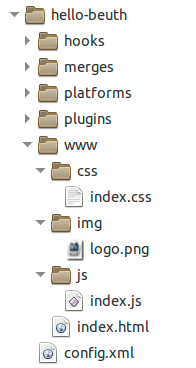
\includegraphics[
%	width=1\textwidth,
	natwidth=1,
	natheight=1,
	resolution=\screenshotRes,
	]{cordova-directory}
	\caption
	[Cordova-Dateistruktur]
	{Dateistruktur einer mit \gls{cordova} erstellten \gls{app}. Das Grundgerüst für die \gls{hybrid-app} wird automatisch angelegt und entspricht den üblichen Web-Entwicklungskonventionen.}
	\label{fig:cordova-directory}
		\imagesourcefont
		\vspace{\imagesourcespace}
		\imagesourcefont{}
		\caption*{\imagesourcelabel Eigener Screenshot.}
\end{figure}
%\end{wrapfigure}

\par\noindent\begin{minipage}{\linewidth}
\lstinputlisting[
	label=lst:config.xml,
%	language=xml,
	style=htmlcssjs, 
	caption={Die Konfigurationsdatei \filename{config.xml}, in der allgemeine Informationen über die \gls{hybrid-app} gespeichert werden. In \linename 2 und 4 tauchen die in \autoref{lst:create} angegebenen optionalen  Parameter \emph{Id} und \emph{Name} wieder auf.},
	]{code/hello-beuth/config.xml}
\end{minipage}\par\addvspace{\topskip}

Die Initialisierung der \gls{app} erfolgt über den \filename{deviceready}-Eventhandler, der standardmäßig von \filename{www/js/index.js} referenziert wird (\seeref{lst:index.html} \linename 40 und \autoref{lst:index.js} \linename 29).


\par\noindent\begin{minipage}{\linewidth}
\lstinputlisting[
	firstline=20,
	lastline=43,
	label=lst:index.html,
	style=htmlcssjs, 
	caption={Startseite der von \gls{cordova} erzeugten \gls{app}, die auf das deviceready-Event reagiert.},
	]{code/hello-beuth/www/index.html}
\end{minipage}\par\addvspace{\topskip}


\par\noindent\begin{minipage}{\linewidth}
\lstinputlisting[
	firstline=19,
	lastline=49,
	label=lst:index.js,
	style=htmlcssjs, 
	caption={Standardmäßig von \gls{cordova} angelegte \gls{js}-Datei \filename{index.js}},
	]{code/hello-beuth/www/js/index.js}
\end{minipage}\par\addvspace{\topskip}

Um die Oberfläche der \gls{app} anzuzeigen, lässt sie sich, da sie im Wesentlichen aus einer \gls{html}-Seite besteht, in einem herkömmlichen Browser öffnen (\seeref{fig:cordova-app-browser}).
Da jedoch das bei der hybriden \gls{app} darunterliegende mobile Betriebssystem hier nicht zur Verfügung steht, ist hier auch keine Anbindung an dessen Funktionalitäten möglich.
Dafür muss die Anwendung entweder direkt auf einem mobilen Gerät, dessen Plattform die \gls{app} und das \gls{cordova}-\gls{api} unterstützen, oder mithilfe eines Emulators ausgeführt werden (\seeref{fig:android_emulate_install}) \cite{Cordova-Docs_CLI}.

\begin{figure}[h!]
\centering
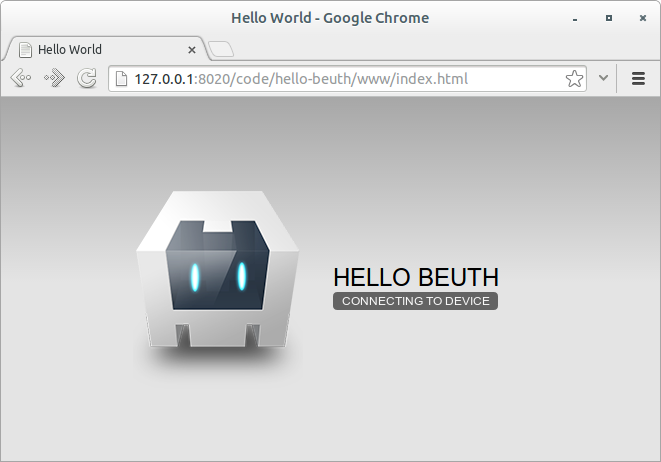
\includegraphics[
	resolution=\screenshotRes,
	natwidth=1,
	natheight=1,
	]{cordova-app-browser}
	\caption
	[\gls{cordova}-Beispiel-\gls{app} im Browser]
	{Die Startseite der Beispiel-\gls{app} aus \autoref{lst:index.html} lässt sich auch im Desktop-Browser öffnen und anzeigen, allerdings kann hier kein \lstinline|deviceready|-Event empfangen werden.}
	\label{fig:cordova-app-browser}
		\imagesourcefont
		\vspace{\imagesourcespace}
		\imagesourcefont{}
		\caption*{\imagesourcelabel Eigener Screenshot.}
\end{figure}

\begin{figure}[h!]
\centering
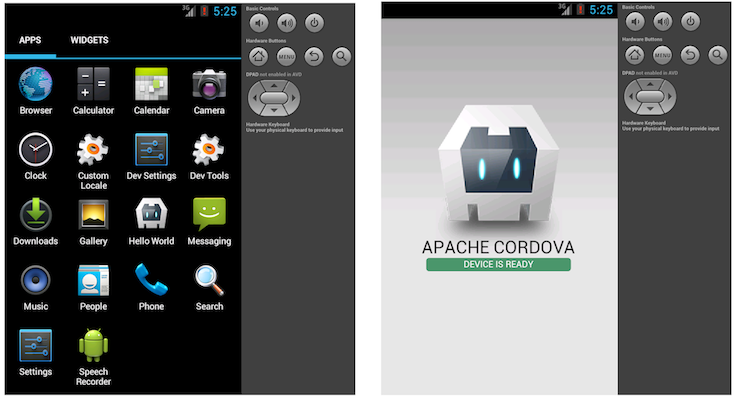
\includegraphics[
	width=1\textwidth,
	natwidth=1,
	natheight=1,
	]{android_emulate_install}
	\caption
	[\gls{cordova}-Beispiel-\gls{app} im \gls{android}-Emulator]
	{Anzeige in der \glspl{app}-Übersicht (links) und Ausführung der \gls{cordova}-Beispiel-\gls{app} in einem \gls{android}-Emulator (rechts). Das grüne Label zeigt den Empfang des \lstinline|deviceready|-Events an.}
	\label{fig:android_emulate_install}
		\imagesourcefont
		\vspace{\imagesourcespace}
		\imagesourcefont{}
		\caption*{\imagesourcelabel \gls{cordova}-Dokumentation \cite{android_emulate_install.png}}
\end{figure}


Befor die \gls{hybrid-app} mit \gls{cordova} zum Laufen gebracht werden kann, muss sie, wie die meisten Computerprogramme, in ein ausführbares Format überführt, also \emph{gebaut} werden.
Im Falle der \gls{hybrid-app} bedeutet das, dass diejenigen plattformspezifischen Komponenten der \gls{app} hinzugefügt werden, die nötig sind, um die Verbindung zwischen der plattformunabhängigen Web-Schicht und der nativen Schicht des jeweiligen Zielbetriebsystems herzustellen.

Damit das \gls{cordova}-Framework die entsprechenden Schnittstellen in die Anwendung einfügen kann, muss vor dem Build-Prozess ein Satz an Zielplattformen angegeben werden. 
Voraussetzung hierfür ist, dass die \glspl{sdk} der jeweiligen Zielplattformen zu der verwendeten Entwicklungsplattform kompatibel installiert sind \cite{Cordova-Docs_CLI}.

Über den \lstinline|cordova|-Befehl \lstinline|platform| lassen sich mit den Optionen \lstinline|add| und \lstinline|remove| Plattformen zur Projekt-Konfiguration der Anwendung hinzufügen bzw. entfernen (\seeref{lst:platform-add-remove}).
Die Ausführung dieser Befehle wirkt sich auf den Inhalt des \filename{platforms}-Ordners innerhalb der Projektstruktur aus \cite{Cordova-Docs_CLI}.

\begin{lstlisting}[
	language=bash,
	caption={\gls{cordova}-Skript um Plattformen zum Projekt hinzuzufügen bzw. zu entfernen. \linename 1 fügt die Plattform \gls{android} hinzu, \linename 2 entfernt diese wieder.},
	label=lst:platform-add-remove]
	$ cordova platform add android
	$ cordova platform remove android
\end{lstlisting}

Um eine Liste aller Plattformen des Projekts auszugeben, dient der \lstinline|list|-Befehl. Wie bei den meisten anderen Befehlen auch, kann synonym auch eine Kurzschreibweise (\lstinline|ls|) verwendet werden.

\begin{lstlisting}[
	language=bash,
	caption={\gls{cordova}-Skript zum Auflisten aller Plattformen des Projekts.},
	label=lst:platform-list]
	$ cordova platforms list
\end{lstlisting}

Anschließend kann mit dem \lstinline|build|-Befehl die \gls{app} gebaut werden:

\begin{lstlisting}[
	language=bash,
	caption={Bauen der \gls{cordova}-\gls{app} für \gls{android}.},
	label=lst:cordova-build]
	$ cordova build android
\end{lstlisting}

Der \lstinline|build|-Befehl stellt dabei eine Kurzform für die beiden Befehle \lstinline|prepare| und  \lstinline|compile| dar (\seeref{lst:prepare-compile}).
Diese Aufteilung kann beispielsweise sinnvoll sein, um erst den \lstinline|prepare|- Befehl auszuführen und den plattformspezischen Code, den Cordova in \filename{platforms/android} generiert, anschließend mit einer entsprechenden \gls{ide} (wie bspw. \gls{android-studio}) und deren nativem SDK anzupassen und zu kompilieren.\footnote{\vgl Nativ-Entwicklungsansatz, \so.}

\begin{lstlisting}[
	language=bash,
	caption={Ausführlichere Schreibweise für den \lstinline|build|-Befehl aus \autoref{lst:cordova-build}.},
	label=lst:prepare-compile]
	$ cordova prepare android
	$ cordova compile android
\end{lstlisting}

Ist der Build-Prozess abgeschlossen, kann die fertige \gls{app} auch mit dem \gls{cordova}-\gls{cli} getestet werden. 
Die Anwendung kann dafür entweder an einen Emulator, der in vielen Fällen mit dem jeweiligen \gls{sdk} mitgeliefert wird, übergeben (\seeref{lst:emulate}) oder direkt auf einem an den Entwicklungsrechner angeschlossenen Mobilgerät ausgeführt werden (\seeref{lst:run}).
Für letzteres müssen unter Umständen noch entsprechende Einstellungen auf dem Gerät vorgenommen werden \cite{Cordova-Docs_CLI}.

\begin{lstlisting}[
	language=bash,
	caption={Übergibt die \gls{app} an den Emulator des \gls{android}-\glspl{sdk}.},
	label=lst:emulate]
	$ cordova emulate android
\end{lstlisting}

\begin{lstlisting}[
	language=bash,
	caption={Führt die \gls{app} auf einem angeschlossenen Mobilgerät aus.},
	label=lst:run]
	$ cordova run android
\end{lstlisting}

Um den eigentlichen Mehrwert des \gls{cordova}-Frameworks zu nutzen, also auf native Features der Zielplattformen zuzugreifen, sind verschiedene Plugins nötig, die ebenfalls mit dem \gls{cli} verwaltet werden können.
\gls{cordova} bietet von Haus aus eine ganze Reihe von Plugins an, es können aber auch eigene entwickelt werden.\footnote{So bietet \zB \gls{adobe} mit seiner \gls{phonegap}-Variante noch einige weitere Plugins wie bspw. den Zugriff auf einen angeschlossenen Barcode-Scanner an, die über die Grundausstattung von \gls{cordova} hinausgehen \cite{Cordova-Docs_CLI}.}

Plugins bestehen aus einem zusätzlichen Stück Code, der die Kommunikation zu den nativen Komponenten herstellt.
Das \gls{cordova}-\gls{cli} bietet auch die Möglichkeit, alle verfügbaren Plugins zu durchsuchen, hinzuzufügen, aufzulisten und zu entfernen (\seeref{lst:plugin-search}, \ref{lst:plugin-add}, \ref{lst:plugin-ls} und \ref{lst:plugin-rm}).

Plugin suchen: 
\begin{lstlisting}[
	language=bash,
	caption={Suchen von verfügbaren Plugins.},
	label=lst:plugin-search]
	$ cordova plugin search contacts
\end{lstlisting}

\begin{lstlisting}[
	language=bash,
	caption={Plugin zur App hinzufügen.},
	label=lst:plugin-add]
	$ cordova plugin add org.apache.cordova.contacts
\end{lstlisting}

\begin{lstlisting}[
	language=bash,
	caption={Analog zum \lstinline|list|-Befehl für Plattformen (\seeref{lst:platform-list}) können auch Plugins des aktuellen Projekts aufgelistet werden.},
	label=lst:plugin-ls]
	$ cordova plugin ls
\end{lstlisting}

\begin{lstlisting}[
	language=bash,
	caption={Plugin entfernen.},
	label=lst:plugin-rm]
	$ cordova plugin rm org.apache.cordova.contacts
\end{lstlisting}




%TODO Referenzen einfügen!!



\subsection{PhoneGap\,Build}

%TODO Welche Plattformen werden von Build unterstützt?

Mit seinem Online-Portal \gls{pg-build} bietet \gls{adobe} einen webbasierten Build-Service für \gls{phonegap}-Apps an, der den Bau-Prozess, im Falle der hybriden \glspl{app} also die eigentliche Anbindung an plattformspezifische Toolkits auf nativer Ebene, auslagert und damit deutlich vereinfacht.
Wie in \autoref{fig:hybrid-apps-schaubild} dargestellt, muss dieser Entwicklungsschritt im Gegensatz zu den vorherigen\footnote{Also der Entwicklung des Codes und der Oberfläche sowie Tests.} trotz (oder gerade wegen) des plattformunabhängigen Charakters mehrfach (also einmal für jede Zielplattform) ausgeführt werden, um die vorher entwickelte Web-App in die Umgebung einer native App einzubetten (\seeref{sec:hybrid-app}). %TODO Auf die unterschiedlichen Entw.-Plattformen eingehen, die nötig sind, um ein möglichst breites Spektrum an Zielplattformen zu erreichen!! -> S. Cordova / PhoneGap [Dieses "mehrfach" hier heißt ja eigentlich nicht zeitlicher mehraufwand, sondern vor allem administrativen!]
Um also nicht auf jedem Entwicklungsrechner sämtliche Toolkits aller Zielplattformen verwalten zu müssen, können \gls{phonegap}-Entwickler hier ihren Quellcode hochladen und die App für die verschiedenen Zielplattformen im jeweiligen Format zusammenbauen bauen lassen.

Um den Build-Prozess über das den Cloud-Build-Service einzuleiten, erstellt der Entwickler eine \gls{web-app} in seiner gewohnten \gls{ide} in Form von \gls{html}-, \gls{js}- und \gls{css}-Dokumenten, die er anschließend auf \gls{pg-build} hochlädt.
Hierfür muss zunächst über die Web-Oberfläche des Portals eine neue \gls{app} angelegt werden.

Abhängig vom jeweiligen Bezahlpaket haben \gls{phonegap}-Entwickler die Möglichkeit, ihre Anwendung als private oder öffentliche \gls{app} hochzuladen. 
Während private \glspl{app} entweder als Zip-Paket hochgeladen oder als Link zu einem \gls{git}-Repository\footnote{Beispielsweise wie die öffentlichen Apps auf \gls{github} gehosted oder einem eigenen \gls{git}-Repository} in \gls{pg-build} eingestellt werden können (\seeref{fig:phonegap-build_create-public}), müssen öffentliche (also \gls{opensource}-) \glspl{app} in Form eines \gls{github}-Repositorys zugänglich gemacht werden.

\begin{quote}
\enquote{We only allow open-source apps to be built from public Github repos} \cite{PhoneGap_Build_Apps}
\end{quote}


\begin{figure}[h!]
\centering
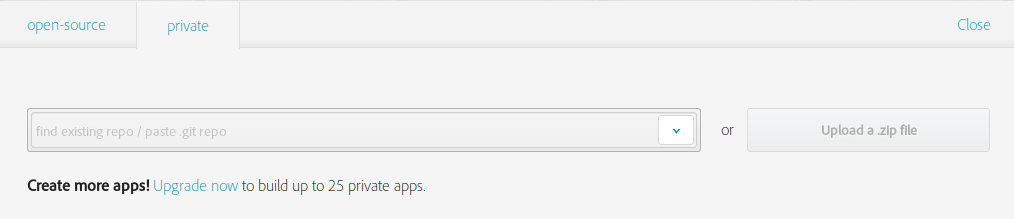
\includegraphics[
	width=1\textwidth,
	natwidth=1,
	natheight=1,
	]{phonegap-build_create-public}
	\caption
		[Erstellung einer neuen App auf \gls{pg-build}]
		{Dialog für die Erstellung einer neuen privaten \gls{app} auf \gls{pg-build}. Links das Eingabefeld zum Eintragen eines \gls{git}-Repository-Links und rechts der Button zum Hochladen von Zip-Archiven.}
		\label{fig:phonegap-build_create-public}
	\imagesourcefont
	\vspace{\imagesourcespace}
	\imagesourcefont{}
	\caption*{\imagesourcelabel Eigener Screenshot.}
\end{figure}


Neben der Bezahlvariante gibt es auch ein kostenloses Paket, das eine private \gls{app} beinhaltet, bei der kostenpflichtigen Variante sind bis zu 25 private App enthalten.
\gls{opensource}-\glspl{app} können bei allen Paketen unbegrenzt angelegt werden (\seeref{fig:phonegap-build_plans}).

\begin{figure}[h!]
\centering
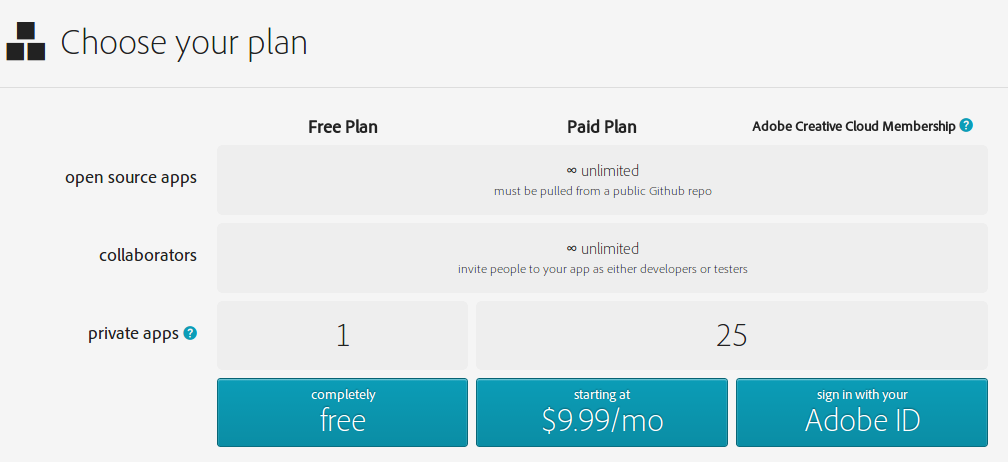
\includegraphics[
	width=1\textwidth,
	natwidth=1,
	natheight=1,
	]{phonegap-build_plans}
	\caption
		[\gls{pg-build}-Pakete]
		{Übersicht über die verschiedenen Bezahlpakete von \gls{pg-build}: Ab 9,99\,\$ im Monat können Entwickler bis zu 25 private \glspl{app} anlegen, in der kostenlosen Variante nur eine private, aber unbegrenzt öffentliche.}
		\label{fig:phonegap-build_plans}
	\imagesourcefont
	\vspace{\imagesourcespace}
	\imagesourcefont{}
	\caption*{\imagesourcelabel Eigener Screenshot \cite{Adobe_PhoneGap_Build_Plans}.}
\end{figure}


Nach dem Hochgeladen des Codes auf \gls{pg-build}, wird dort automatisch der Build-Prozess für die \glspl{hybrid-app} initiiert.
Dabei sorgt \gls{pg-build} dafür, dass für jede Plattform die entsprechende \gls{phonegap}-\gls{js}-Bibliothek injiziert wird, welche die \gls{api} zur nativen Betriebssystemebene enthält (\seeref{sec:phonegap}) \cite{PhoneGap_Build_Documentation_getting-started}.
Ist der Build-Prozess abgeschlossen, kann die \gls{app} im jeweiligen Format für die verschiedenen Plattformen als Direkt-Link oder per \gls{qr} heruntergeladen werden (\seeref{fig:phonegap_build_workflow} und \ref{fig:phonegap-build_apps}).

\begin{figure}[h!]
\centering
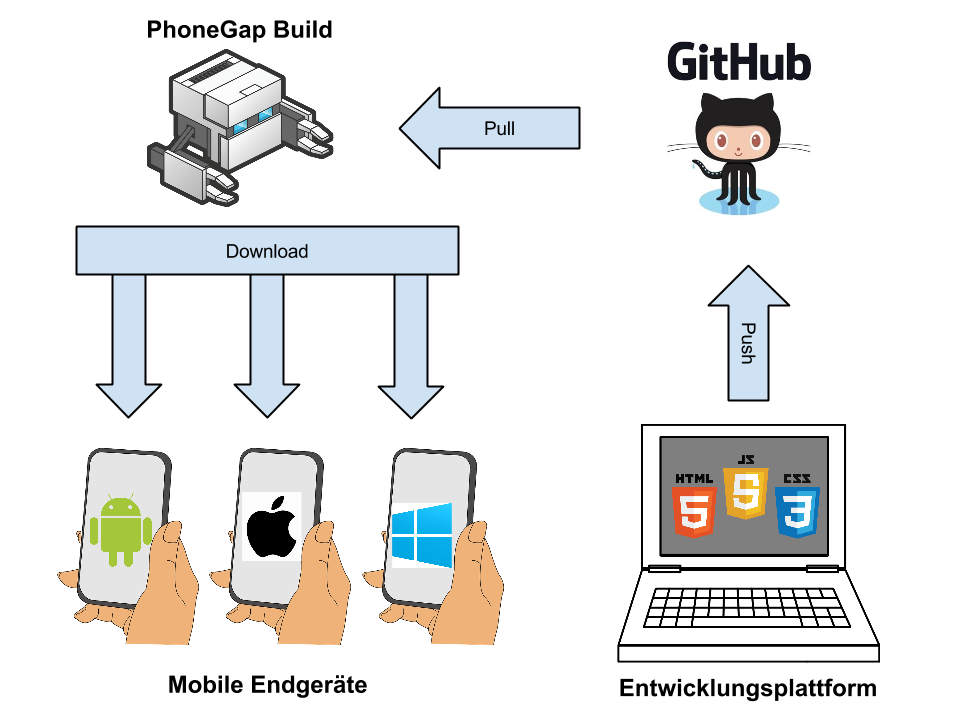
\includegraphics[
	width=1\textwidth,
	natwidth=1,
	natheight=1,
	]{PhoneGap_Build_Workflow}
	\caption[\gls{pg-build}-Workflow]{Schematische Darstellung eines möglichen Entwicklungsworkflows mit \gls{pg-build}: Der Code wird als Web-Anwendung auf \gls{github} hochgeladen, bei \gls{pg-build} über das \gls{github}-Repository aktualisiert und für die jeweiligen Plattformen gebaut, sodass die plattformspezifischen \glspl{app} heruntergeladen und auf den Zielgeräten installiert werden können.}
	\label{fig:phonegap_build_workflow}
	\imagesourcefont
	\vspace{\imagesourcespace}
	\imagesourcefont{}
	\caption*{\imagesourcelabel Eigene Grafik.}
\end{figure}
%TODO Als SVG einbinden! -> Funzt noch nicht.
%TODO Bildquellen (innerhalb des Bilder angeben.)


\begin{figure}[h!]
\centering
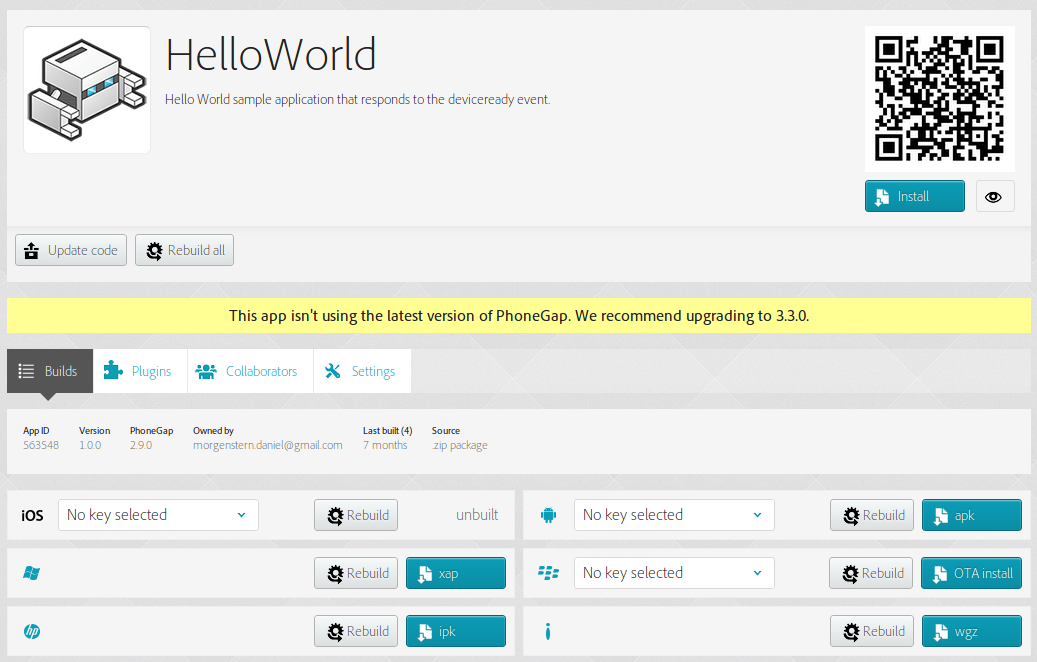
\includegraphics[
	width=1\textwidth,
	natwidth=1,
	natheight=1,
	]{phonegap-build_apps}
	\caption[\gls{pg-build}-Oberfläche]{Oberfläche des \gls{pg-build}-Portals: Detailansicht für eine Beispiel-\gls{app}. Hier können verschiedene Einstellungen vorgenommen werden, sowie der Code aus einem Repository aktualisiert und die fertig gebaute \gls{app} per Download-Button oder \gls{qr} heruntergeladen werden.}
	\label{fig:phonegap-build_apps}
	\imagesourcefont
	\vspace{\imagesourcespace}
	\imagesourcefont{}
	\caption*{\imagesourcelabel Eigener Screenshot.}
\end{figure}

\begin{figure}[h!]
\centering
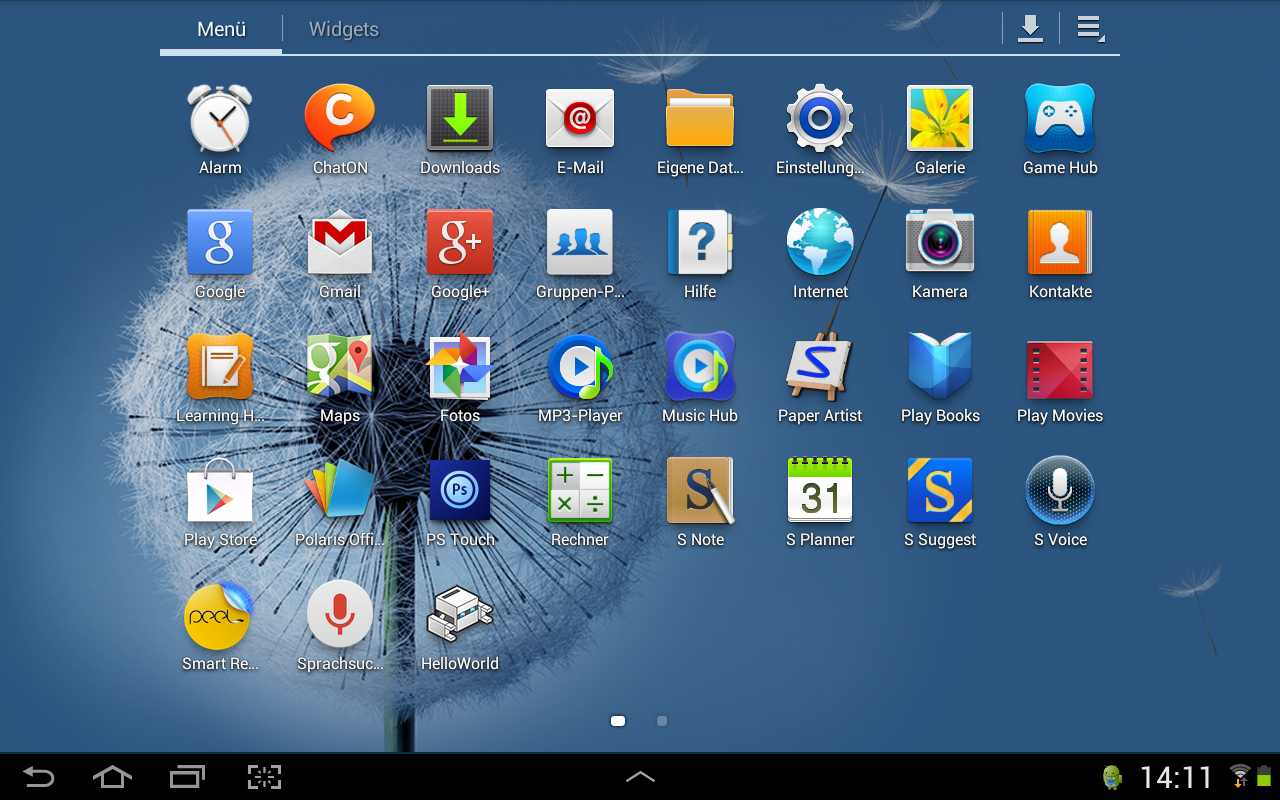
\includegraphics[
	width=1\textwidth,
	natwidth=1,
	natheight=1,
	]{screenshot_app_android}
	\caption
	[Tablet-Screenshot mit installierter \gls{phonegap}-\gls{app}]
	{Die Beispiel-App (\enquote{HelloWorld}) aus \autoref{fig:phonegap-build_apps} aus \gls{pg-build} auf einem \gls{android}-Gerät installiert.}
	\label{fig:screenshot_app_android}
	\imagesourcefont
	\vspace{\imagesourcespace}
	\imagesourcefont{}
	\caption*{\imagesourcelabel Eigener Screenshot.}
\end{figure}


%TODO Evtl. Screenshot Test-App im Desktop-Browser und dann als mobile App.

